
We need to introduce anyons here, or somehow build it into the review of the golden chain.

This chapter the diagrammatic methods that yield tensor networks on physical systems that
constitute \emph{anyons}. We introduce the fundamental theory of anyons algebraically
(\Cref{anyon:sec:algebraic_theory_of_anyons}), and make use of the algebraic rules as the
building blocks for our theory. \Cref{anyon:sec:topology} gives examples of how the
statistical properties of anyons change with respect to it's ground state. Then, in
\Cref{anyon:sec:lattice_spin_chains}, we provide a worked examples of how anyons are
treated on \emph{spin-chains}, which motivates some aspect of the tensor networks
approach. TODO tensor network chapter. One of the primary motivations for the study of
anyons are their universality for quantum computation. In
\Cref{anyon:sec:tqc} we provide an interpretation of how both
normal braiding circuits and a variation in terms of \emph{weaves} can be simulated by the
tensor network theory.

\section{Algebraic Theory of Anyons}\label{anyon:sec:algebraic_theory_of_anyons}

Anyons are proposed as a \emph{defect} in a $2$ dimensional space (manifold? compact?)
with exotic exchange statistics. These exchange statistics differ from fermions in that we
allow particles to pick up a arbitrary phase $e^{i\theta}$ on exchange in the abelian
case, and a phase in a matrix element in the nonabelian case.

Generally when speaking about anyons, we group them into \emph{theories}. A anyon theory
is equipped with a (finite) set of charges $a,b,c,\ldots$ including a \emph{vacuum} charge
$I$. Additionally we are provided with a \emph{fusion rule} $a \times b = \sum_{c}^{}
N_{ab}^c c$ where $N_{ab}^c$ denotes the multiplicity. Since it can be shown (should I?)
that we cannot classify the vector space of two anyons $a,b$ by itself, we need to
parametrize this space over its \emph{fusion sectors}, i.e. the outcomes $c$ of the fusion
rule.

Consider an anyon to be a point-like defect on the plane carrying a charge out of the set
of labels. Since we need to reason about the properties of a pair of anyons using their
fusion-outcome, we draw this as follows:
%\[
%  \begin{tikzpicture}[scale=1.5]
%    \fill[gray!30] (3,0) ellipse (1 and 0.5);
%    \draw[->, thick] (3,0) ellipse (1 and 0.5);
%    \fill[white] (3.6,0) circle (0.1);
%    \draw[->, thick] (2.7,0) ellipse (0.6 and 0.3);
%    \node at (3.35,-0.2) {$1$};
%    \node[scale=2.5] at (2.4, 0) {$\cdot$};
%    \node at (2.5,0.1) {$\tau$};
%    \node[scale=2.5] at (3.0, 0) {$\cdot$};
%    \node at (3.1,0.1) {$\tau$};
%    \node[scale=2.5] at (3.6, 0) {$\cdot$};
%    \node at (3.7,0.1) {$\tau$};
%    \node at (4.0,-0.3) {$\tau$};
%\end{tikzpicture}
%\]
\[
  \begin{tikzpicture}[scale=1,
    ->-/.style={decoration={
      markings,
      mark=at position #1 with {\arrow[scale=1.5]{>}}},postaction={decorate}}
    ]

    \fill[gray!15] (1.5, 0) ellipse (2.4 and 1.2);
    \draw[thick, ->-=0.55] (1.5, 0) ellipse (2.4 and 1.2);
    \node at (2.4, -0.8) {$\tau$};

    \fill[gray!30] (0.75, 0) ellipse (1.2 and 0.6);
    \draw[thick, ->-=0.55] (0.75, 0) ellipse (1.2 and 0.6);
    \node at (0.75, -0.35) {$1$};

    \fill[black] (0, 0) circle (1.5pt);
    \node at (0, 0.25) {$\tau$};

    \fill[black] (1.5, 0) circle (1.5pt);
    \node at (1.5, 0.25) {$\tau$};

    \fill[black] (3.0, 0) circle (1.5pt);
    \node at (3.0, 0.25) {$\tau$};

\end{tikzpicture}
\]
The thick dark ellipses here denote the fusion outcome of two charges. Note that the line
here has an additional physical property in such that it is an \emph{observable}. This has
a nice interpretation in terms of bordisms: 

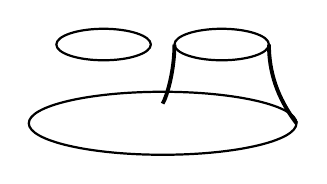
\begin{tikzpicture}
  \draw[thick] (3.25,0) ellipse (1.7 and 0.4);
  \draw[thick] (2.5,1) ellipse (0.6 and 0.2);
  \draw[thick] (4,1) ellipse (0.6 and 0.2);

  \draw[line width=1.4] (4.95, 0) .. controls (4.7, 0.33) and (4.6, 0.66) .. (4.6, 1);
  \draw[line width=1.4] (3.25, 0.25) .. controls (3.3, 0.33) and (3.4, 0.66) .. (3.4, 1);

\end{tikzpicture}

\[
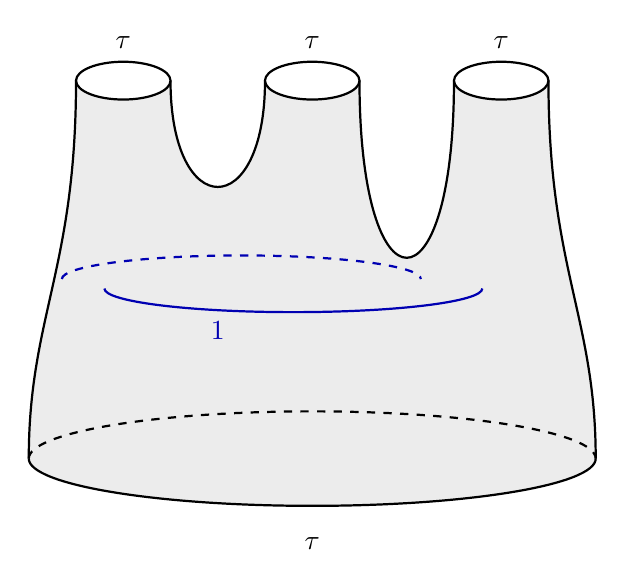
\begin{tikzpicture}[scale=1.2, thick]
    
    \fill[gray!15]
        (-2.5,0)
        .. controls (-2.5,1.5) and (-2,2) .. (-2,4)
        arc (180:360:0.5 and 0.2)
        .. controls (-1,2.5) and (0,2.5) .. (0,4) 
        arc (180:360:0.5 and 0.2)
        .. controls (1,1.5) and (2,1.5) .. (2,4)
        arc (180:360:0.5 and 0.2) 
        .. controls (3,2) and (3.5,1.5) .. (3.5,0) 
        arc (360:180:3.0 and 0.5);

    \draw (-2.5,0) .. controls (-2.5,1.5) and (-2,2) .. (-2,4);
    \draw (3.5,0)  .. controls (3.5,1.5) and (3,2) .. (3,4);
    
    \draw (-1,4) .. controls (-1,2.5) and (0,2.5) .. (0,4);
    \draw (1,4)  .. controls (1,1.5) and (2,1.5) .. (2,4);

    \draw[dashed, blue!70!black, thick] (-2.15, 1.9) arc (180:0:1.9 and 0.25);
    \draw[blue!70!black, thick] (-1.7, 1.8) arc (180:360:2.0 and 0.25
);
    \node[blue!70!black] at (-0.5, 1.35) {$1$};


    \fill[white] (-1.5,4) ellipse (0.5 and 0.2);
    \draw (-1.5,4) ellipse (0.5 and 0.2);
    \node at (-1.5, 4.4) {$\tau$};

    \fill[white] (0.5,4) ellipse (0.5 and 0.2);
    \draw (0.5,4) ellipse (0.5 and 0.2);
    \node at (0.5, 4.4) {$\tau$};

    \fill[white] (2.5,4) ellipse (0.5 and 0.2);
    \draw (2.5,4) ellipse (0.5 and 0.2);
    \node at (2.5, 4.4) {$\tau$};

    \draw[dashed] (-2.5,0) arc (180:0:3.0 and 0.5);
    \draw (-2.5,0) arc (180:360:3.0 and 0.5);
    \node at (0.5, -0.9) {$\tau$};

\end{tikzpicture}
\]



Let $V^{ab}_c$ be the space of 2 anyons of charges $a,b$ fusing to $c$. Then the

whole space $V^{ab}$ splits accordingly:
\[
  V^{ab} = \bigoplus_{c \in I} V^{ab}_c . 
\]
Since we wanted to assign meaning to the \emph{exchange} of particles, we define the exchange operator $R^{ab}$ componentwise:
\[
  R^{ab} : V^{ab} \to V^{ba}, \quad \bigoplus_c V^{ab}_c \cong \bigoplus_c V^{ba}_c.   
\]
as well as an isomorphism on combinations of more than $3$ particles
\[
  F^{abc} : V^{(ab)c} \cong V^{a(bc)}
\]

\subsection{Anyons on different topologies}\label{anyon:sec:topology}


\begin{figure}[h]
  \centering
  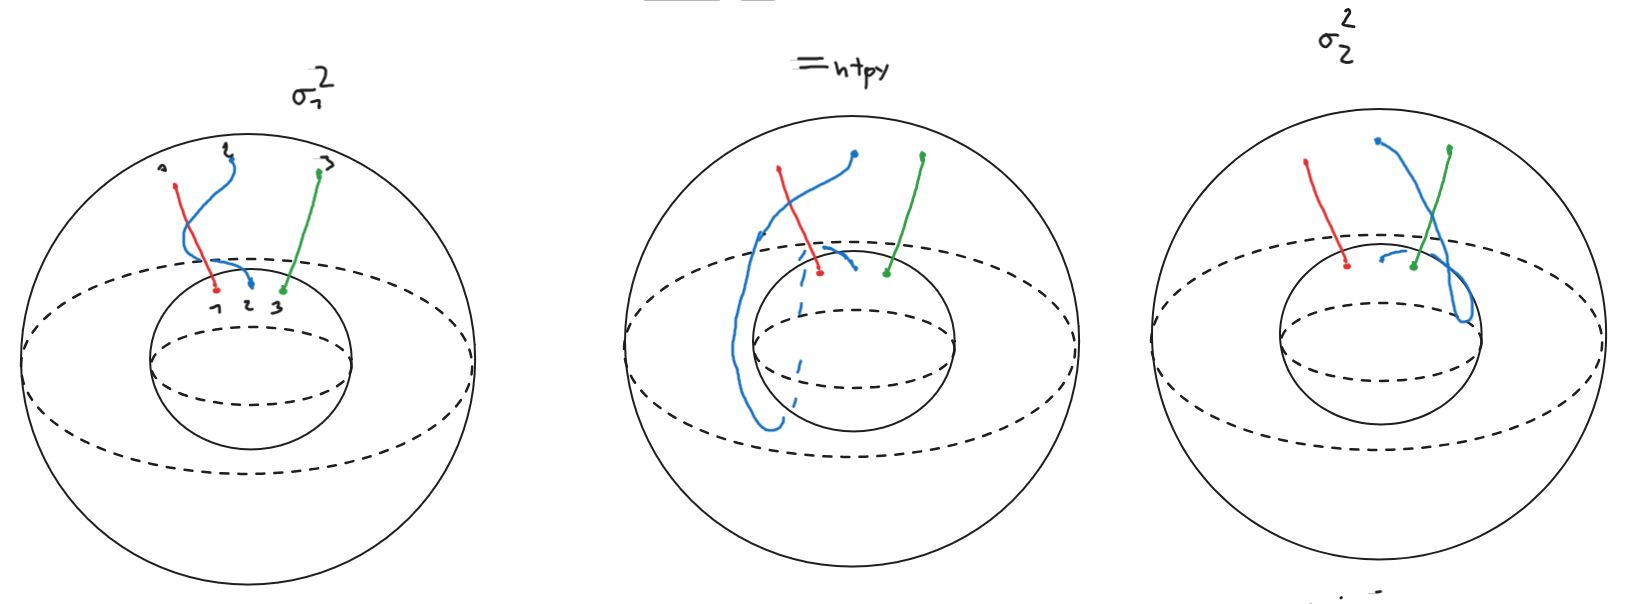
\includegraphics[width=0.8\textwidth]{figures/anyons_sphere.png}
  \caption{ $3$ Anyons on the sphere $S^2$ with the equivalence of the braids $\sigma_1^2$
    and $\sigma_2^2$. From an
    exercise\href{https://github.com/jkr11/maths-notes/tree/main/tq-simons-solutions}{github}
    in \cite{simonTopologicalQuantum2023}. }
  \label{anyon:fig:sphere}
\end{figure}

Analysing this case further yields that 
\[
  \pi_1(\mathrm{Conf}_3(S^2)) \cong Br(S^2) \cong \Z_4 \boxtimes \Z_3
\]
and thus finite. In fact, we know about the braid group on spheres that the order of
$Br_n(S^2)$ is given by
\begin{equation}
  \left\vert Br_n(S^2) \right\vert = \begin{dcases}
    \left\vert \Z_2 \right\vert = 2 &\text{ if } n = 2,\\
    \left\vert ??? \right\vert = 12  &\text{ if } n = 3, \\
    \infty &\text{ if } n \geq 4.
  \end{dcases}
  %\text{
  %  \stackrel{\cite[P~255]{fadellBraidGroupsE21962}}{\cite[Prop~2.2]{nlab:spherical_braid_group}}
  %}
  \shortstack[l]{
    \cite[p.~255]{fadellBraidGroupsE21962} \\
    \cite[Prop~2.2]{nlab:spherical_braid_group}
  }
\end{equation}


Also we should do or have done isotopy before. Technically the discussion here also
requires the completeness relations.

\begin{equation}\label{anyon:eq:complete}
\begin{tikzpicture}[
    baseline=(current bounding box.center),
    scale=1.0,
    string arrow/.style={
        postaction={decorate},
        decoration={
            markings,
            mark=at position 0.55 with {\arrow[scale=1.0]{Stealth}}
        }
    }
  ]
  
  \draw[string arrow] (-2.5, 1.0) -- (-2.5, 3.0) node[above] {$a$};
  \draw[string arrow] (-1.9, 1.0) -- (-1.9, 3.0) node[above] {$b$};

  \node at (-1.1, 2.0) {$=$};
  \node at (-0.1, 2.0) {$\displaystyle\sum_{c,\mu} \sqrt{\frac{d_c}{d_a d_b}} $};

  \coordinate (bot_a) at (1.1, 1.0);
  \coordinate (bot_b) at (2.1, 1.0);
  
  \coordinate (mid_bot) at (1.6, 1.6);
  \coordinate (mid_top) at (1.6, 2.4);
  
  \coordinate (top_a) at (1.1, 3.0);
  \coordinate (top_b) at (2.1, 3.0);

  \draw[string arrow] (bot_a) -- (mid_bot);
  \draw[string arrow] (bot_b) -- (mid_bot);
  
  \draw[string arrow] (mid_bot) -- (mid_top) node[right, pos=0.5] {$c$};
  
  \draw[string arrow] (mid_top) -- (top_a) node[above] {$a$};
  \draw[string arrow] (mid_top) -- (top_b) node[above] {$b$};

\end{tikzpicture}
\end{equation}

\section{1D Lattice Models \& The Golden Chain}\label{anyon:sec:lattice_spin_chains}

%So from what i can read here (also the nlab or wikipedia) a spin chain specifically only
%refers to a per site construction with a tensor product hilbert space. An anyon chain is,
%well, an anyonic chain. These do not admit such a decomposition. So we should call these
%simply 1D lattice models.

In \cite{feiguinInteractingAnyonsTopological2007}, anyonic chains, specifically in the
$\Fib$ model, are introduced as a $1$D lattice of $n$ $\tau$ anyons, defined as the fusion
space thereof.

\begin{tikzpicture}[
    baseline=(current bounding box.center),
    scale=1.2,
    string arrow/.style={
        postaction={decorate},
        decoration={
            markings,
            mark=at position 0.55 with {\arrow[scale=1.0]{Stealth}}
        }
    }
]
  \node (tleft) at (-3.9, 2.7) [left] {$\tau$};
  \node (t1) at (-3.2, 3.2) [above] {$\tau$};
  \node (t2) at (-2.5, 3.2) [above] {$\tau$};
  \node (t3) at (-1.8, 3.2) [above] {$\tau$};
  \node at (-0.5, 3.2) {$\cdots$};
  \node (tn1) at (0.8, 3.2) [above] {$\tau$};
  \node (tn) at (1.6, 3.2) [above] {$\tau$};

  \node (xi1) at (-3.2, 2.7) [inner sep=0pt, label=below:{$x_1$}] {};
  \node (xi2) at (-2.5, 2.7) [inner sep=0pt, label=below:{$x_2$}] {};
  \node (xi3) at (-1.8, 2.7) [inner sep=0pt, label=below:{$x_3$}] {};

  \draw [string arrow] (tleft) -- (xi1);
  \draw [string arrow] (t1) -- (xi1);

  \draw [string arrow] (t2) -- (xi2);
  \draw [string arrow] (xi1) -- (xi2);

  \draw [string arrow] (t3) -- (xi3);
  \draw [string arrow] (xi2) -- (xi3);

\end{tikzpicture}

Here, the state is fully characterized by its intermediate indeces $x_1 \ldots x_{n-1}$,
so we can choose a basis $\ket{x_1 x_2 \cdots x_{n-1} }$.

Similar to the Heisenberg-chain\footnote{Note that $\frac{1}{2} \otimes \frac{1}{2} = 0
\oplus 1$ in the Heisenberg $\SU 2$ model.}, the golden chain introduces a Hamiltonian
that assigns $-1$ to the interaction $\tau \otimes \tau = 1$ and $0$ to the interaction
$\tau \otimes \tau = \tau$.

We can decompose the whole space $\Hom(\tau^{\otimes n+1}, \tau)$ into the local states
\begin{equation}
  \Hom(\tau^{\otimes n+1}, \tau) 
  =
  \bigoplus_{\mathclap{\substack{x_1, x_2, \ldots, x_{n-1} \\ \text{\color{RoyalBlue}{all admissible paths}}}}}
  \Hom(\tau \otimes \tau, x_1) \otimes \Hom(x_1 \otimes \tau, x_2)
  \otimes \cdots \otimes Hom(x_{n-1} \otimes \tau, \tau) 
\end{equation}
with the admissability condition that there are not adjacents $1$ in the sequence of
$x_i$s.

This is evaluated as a $3$ local hamiltonian, as we can decompose the spin chain into
local parts where two $\tau$ anyons are adjacent (check how they call it in the paper.).

\begin{tikzpicture}[
    baseline=(current bounding box.center),
    scale=1.2,
    string arrow/.style={
        postaction={decorate},
        decoration={
            markings,
            mark=at position 0.55 with {\arrow[scale=1.0]{Stealth}}
        }
    }
]
  \coordinate (tleft) at (-3.9, 2.7);
  \node (t1) at (-3.2, 3.2) [above] {$\tau$};
  \node (t2) at (-2.5, 3.2) [above] {$\tau$};
  
  \coordinate (v1) at (-3.2, 2.7);
  \coordinate (v2) at (-2.5, 2.7);
  \coordinate (v3) at (-1.8, 2.7);

  \draw [string arrow] (tleft) -- node[below] {$x_{i-1}$} (v1);
  \draw [string arrow] (t1) -- (v1);

  \draw [string arrow] (v1) -- node[below] {$x_{i}$} (v2);
  \draw [string arrow] (t2) -- (v2);
  
  \draw [string arrow] (v2) -- node[below] {$x_{i+1}$} (v3);

  %\node (in1) at (-2.5, 2.0) {\tiny $\in Hom(x_{i-1} \otimes \tau, x_i)$ \\ $\otimes Hom(x_i \otimes \tau, x_{i+1} )$}; 
  \node (in1) at (-2.5, 1.8) [align=center] {
    \small $\in \Hom(x_{i-1} \otimes \tau, x_i)$ \\ 
    \small $\otimes \Hom(x_i \otimes \tau, x_{i+1})$
  };


  \node at (-1.3, 2.9) {$=$};
  \node at (-0.3, 2.8) {$\displaystyle\sum_{x_i} [F^{x_{i-1}\tau \tau }_{x_{i+1}}]_{\blue{x_i}}^{\blue x_i^\prime} $};

  \begin{scope}[xshift=4.6cm]
    \coordinate (rtleft) at (-3.9, 2.7);
    \node (rt1) at (-3.2, 3.2) [above] {$\tau$};
    \node (rt2) at (-2.5, 3.2) [above] {$\tau$};
    \coordinate (rtright) at (-1.8, 2.7);
    
    \coordinate (rvtau) at (-2.85, 2.95);
    
    \coordinate (rv1) at (-2.85, 2.7);

    \draw [string arrow] (rtleft) -- node[below] {$x_{i-1}$} (rv1);
    
    \draw [string arrow] (rt1) -- (rvtau);
    \draw [string arrow] (rt2) -- (rvtau);
    
    \draw [string arrow] (rvtau) -- node[left] {$x_{i}^\prime $} (rv1);
    
    \draw [string arrow] (rv1) -- node[below] {$x_{i+1}$} (rtright);

    \node (in1) at (-2.5, 1.8) [align=center] {
      \small $\in \Hom(x_{i-1} \otimes x_i^\prime , x_{i+1} )$ \\
      \small $\otimes \Hom(\tau \otimes \tau, x_{i}^\prime  )$
    }; 

  \end{scope}

\end{tikzpicture}

Now we can apply the interaction based on the intermediate state\footnote{Technically we
need a projector here read up again.} $x_i^\prime$ and apply another $F$-move back to the
chain basis.

\[
  H_{[i,i+1]} : \ket{x_{i-1} x_i x_{i+1}  } \to \ket{x_{i-1} x_i^{\prime\prime} x_{i+1} } \coloneqq  - \sum_{x_i^\prime \in \{1,\tau\} }^{} [F_{x_{i+1} }^{x_{i-1}\tau\tau}]_{x_i}^{x_i^\prime } E_{x_{i}^\prime } [F_{x_{i+1} }^{x_{i-1}\tau\tau }]_{x_{i^\prime }}^{x_{i^{\prime\prime}}}
\]

Write this three local hamiltonian in an operator form
\[
  H_i = -J \begin{pmatrix}
    1 &  &  &  &   \\
     & 0 &  &  &   \\
     &  & 0 &  &   \\
     &  &  & \varphi^{-2}  & \varphi^{-\frac{3}{2}}  \\
     &  &  & \varphi^{-\frac{3}{2}} & \varphi^{-1}    \\
  \end{pmatrix}
\]


This method is reviewed and extended in \cite{trebstShortIntroductionFibonacci2008a}, with
longer ranger interaction. It will become apparent that the construction given in these
papers is a manualization of the tensor network constructions we will build here.
Generalizations to arbitrary models are given in \cite{gilsAnyonicQuantumSpin2013} as well
as \cite{buicanAnyonicChainsTopological2017}. Generalized spin chains and dualities using
module categories are given in \cite{eckQuantumLatticeModels2025}.

The tensor network formalism is handled in \cite{pfeiferSimulationAnyonsTensor2010},
\cite{pfeiferSimulationAnyonsUsing2012} and \cite{ayeniStudiesBraidedNonAbelian2017}, and
in terms of categories this is done in \cite{dissertation} and
\cite{devosTensorKitjlJuliaPackage2025}.

For the tensor network operations, we should consider the changing of the basis as an
implicit operation that is performed when contracting, just like it would be in a normal
einsum.


In a tensor network formalism can build this as an anyonic operator in $Hom(\tau \otimes \tau, \tau \otimes \tau)$ as
\[
  \begin{tikzpicture}[scale=1.2,
    every node/.style={font=\small},
    fusion/.style={circle,fill=black,inner sep=1.2pt}
]

\node at (-2, 0.5) {$H_i = $};

\node at (-1, 0.5) {$E_1$};

\begin{scope}
  \node[fusion] (v1) at (0,0) {};
\node[fusion] (v2) at (0,1) {};

\draw (v1) -- (-0.7,-1);
\draw (v1) -- (0.7,-1);

\draw (v2) -- (0.7,2);
\draw (v2) -- (-0.7,2);

\draw (v1) -- (v2);

\node[left]  at (-0.7,-1) {$\tau$};
\node[right] at (0.7,-1) {$\tau$};
\node[left]  at (-0.7,2) {$\tau$};
\node[right] at (0.7,2) {$\tau$};

\node[left] at (-0.15,0.5) {$1$};

\end{scope}

\node at (1.5,0.5) {$+$};

\node at (2, 0.5) {$E_\tau$};

\begin{scope}[xshift=3cm]
  \node[fusion] (v1) at (0,0) {};
  \node[fusion] (v2) at (0,1) {};

  \draw (v1) -- (-0.7,-1);
  \draw (v1) -- (0.7,-1);

  \draw (v2) -- (0.7,2);
  \draw (v2) -- (-0.7,2);

  \draw (v1) -- (v2);

  \node[left]  at (-0.7,-1) {$\tau$};
  \node[right] at (0.7,-1) {$\tau$};
  \node[left]  at (-0.7,2) {$\tau$};
  \node[right] at (0.7,2) {$\tau$};

  \node[left] at (-0.15,0.5) {$\tau$};

\end{scope}

\end{tikzpicture}
\]
(Note this is allowed due to $\C$-linearity of $\Fib$.)


In this case we can view the golden chain approach chosen above as a manualization of the
tensor network process.

We can also write $H_i$ in its operator form matrix as
\[
  H_{i} \in \bigoplus_{a \in 1,\tau} Hom(\mathbb{C}, \mathbb{C})
\]
as 
\[
  H_i = -J \begin{array}{r@{\hspace{0.5em}}c}
  & \begin{array}{cc} 1 & \tau \end{array} \\
  \begin{array}{r} 1 \\ \tau \end{array} & 
  \begin{pmatrix}
   E_1 & 0\\
   0 & E_\tau   \\
  \end{pmatrix}
\end{array}
\]


\subsection{Topological Entanglement Entropy}

For simple lattice states, \cite{singhMatrixProductStates2014} defines a bipartition of
the lattice into anyons $A$ and $B$. Then we consider the whole space under charge
$a_{tot}$ as
\[
  V_{a_{tot}} = \bigoplus_{N_{ab}^{a_{tot} } = 1} (V^{A}_a \otimes V^{B}_b)
\] 
What i dont get here is why we are allowed to tensor both these sectors together without
the space $V_{ab}^{a_{tot} }$ explicitely.

TODO delete all of this and introduce this over the Hom category.

Anyhow, the fundamental building blocks we are using are the vector spaces $V^{ab}_c$
(where we refer to this as the fusion space from types $a$ and $b$ to $c$). This allows us
to build the vector space of two anyonic types $a,b$ as the sum over the fusion outcome:
\[
  V^{ab} = \bigoplus_{c \in Irr(C)} V^{ab}_c  
\]

We can directly introduce the $R$ move (a braiding of the initial anyons) to obtain the
isomorphic space $V^{ba}$ as
\[
  R : \bigoplus_{c \in Irr(C)} V^{ab}_c  \cong \bigoplus_{c \in Irr(C)} V^{ba}_c  
\] 

We can also write the space $V^{ab}_c = Hom(a \otimes b, c)$ in the categorical language.
Here we also need to realize that there is a difference between the isomorphism $\beta$
and the action of $R$, which is really on the hom space $\Hom(-, c)$. So this would be a
yoneda perspective? Since we know $R$ for all $a,b,c \in C$, we also know the action of
$R$ as an isomorphism. Well technically i believe that this allows us to determine for all
simples $c$, and then semisimplicity extends this to all subjects (this would be nice to
write down) and then the yoneda embedding is enough to know the whole space. Similarly, in
our Rep(G) categories (which i actually belive to be symmetric? Find this in etingof) 

The algebra-category correspondence in the theory of anyons was first noted by
\cite[App~E]{kitaevAnyonsExactlySolved2006}

\section{Topological Quantum Computation}\label{sect:anyon:tqc}

We want to build a quantum computer that acts purely on the topological data provided by the anyon theories, or as named by \textcite{freedmanNPQuantumField1998}, a \emph{Quantum Field Computer}. To do this we need 3 things:

\begin{enumerate}
  \item[] A ground state that has high enough dimension to represent a quantum bit, i.e. is $\cong \C^2$.
  \item[] A option to time evolve the system by application of unitaries.
  \item[] An option to read out the information of the evolved state (\emph{measurement}).
\end{enumerate}




Computing with nonabelian anyons requires a universal gate set built from representations
of the \emph{braid-group}:
\begin{align}
  \sigma_i\sigma_j &= \sigma_j\sigma_i, \;\; \left\vert i - j \right\vert \geq 2 \label{eq:al1}\\
  \sigma_i\sigma_{i+1}\sigma_{i} &= \sigma_{i+1}\sigma_i\sigma_{i+1}, \;\; i \in [1,n-2] \label{eq:al2}
\end{align}\label{eq:artin}
and also the \emph{pure-braid-group}:

By the construction of anyon chains in \Cref{anyon:sec:algebraic_theory_of_anyons}, we know that the space of $3$ anyons fusing to $\tau$ is in fact $2$-dimensional. This motivates a choice of qubits as the following:

\begin{equation*}
  \vert 0 \rangle =
\raisebox{-20pt}{
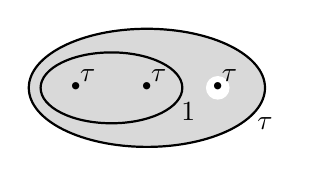
\begin{tikzpicture}[scale=1.5]
    \fill[gray!30] (3,0) ellipse (1 and 0.5);
    \draw[->, thick] (3,0) ellipse (1 and 0.5);
    \fill[white] (3.6,0) circle (0.1);
    \draw[->, thick] (2.7,0) ellipse (0.6 and 0.3);
    \node at (3.35,-0.2) {$1$};
    \node[scale=2.5] at (2.4, 0) {$\cdot$};
    \node at (2.5,0.1) {$\tau$};
    \node[scale=2.5] at (3.0, 0) {$\cdot$};
    \node at (3.1,0.1) {$\tau$};
    \node[scale=2.5] at (3.6, 0) {$\cdot$};
    \node at (3.7,0.1) {$\tau$};
    \node at (4.0,-0.3) {$\tau$};
\end{tikzpicture}
} 
\quad
\vert 1 \rangle = 
\raisebox{-20pt}{
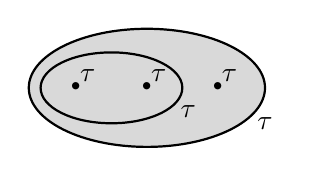
\begin{tikzpicture}[scale=1.5]    
    \fill[gray!30] (3,0) ellipse (1 and 0.5);
    \draw[thick] (3,0) ellipse (1 and 0.5);
    
    \draw[thick] (2.7,0) ellipse (0.6 and 0.3);
    \node at (3.35,-0.2) {$\tau$};

    \node[scale=2.5] at (2.4, 0) {$\cdot$};
    \node at (2.5,0.1) {$\tau$};
    \node[scale=2.5] at (3.0, 0) {$\cdot$};
    \node at (3.1,0.1) {$\tau$};
    \node[scale=2.5] at (3.6, 0) {$\cdot$};
    \node at (3.7,0.1) {$\tau$};
    \node at (4.0,-0.3) {$\tau$};
\end{tikzpicture}
}
\quad 
\vert NC \rangle =
\raisebox{-20pt}{
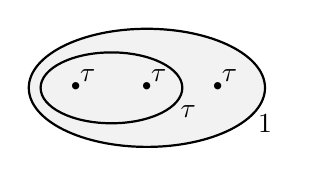
\begin{tikzpicture}[scale=1.5]

    \fill[gray!10] (3,0) ellipse (1 and 0.5);
    \draw[thick] (3,0) ellipse (1 and 0.5);
    
    \draw[thick] (2.7,0) ellipse (0.6 and 0.3);
    \node at (3.35,-0.2) {$\tau$};
    \node[scale=2.5] at (2.4, 0) {$\cdot$};
    \node at (2.5, 0.1) {$\tau$};
    \node[scale=2.5] at (3.0, 0) {$\cdot$};
    \node at (3.1,0.1) {$\tau$};
    \node[scale=2.5] at (3.6, 0) {$\cdot$};
    \node at (3.7,0.1) {$\tau$};
    \node at (4.0,-0.3) {$1$};

\end{tikzpicture}
}
\end{equation*}
and we say that $\C^2$ is \emph{embedded} in $V^{\tau \tau \tau}$. We could choose a different presentations, where each anyon is drawn from the vacuum as
\[
  TODO!
\]

Then we can build multi-qubit circuits by simply stacking these diagrams (inside their own fusion channel). This is what is called a \emph{sparse-encoding}. A dense encoding would correspond to just choosing the smallest space of appropriate dimension that includes one of the $(\C^2)^{\otimes d}$.

The solovay-kitaev theorem guarantees a polylog time and space algorithm for approximating
any gate in $\SU d$ to a desired accuracy. This, and similar procedures are realized by
the functor $\texttt{compile}$. A \emph{topological quantum compiler} essentially only
translates the qubits to their $\Hom$ space equivalences and translates the qudit-gates to
their braid group representations. There are of course special compilation methods, the
one we cover here takes first a decomposition of normal gates into CNOTs and then applies
injection weaving, so we only need to lower single qubit gates to braids.

% https://q.uiver.app/#q=WzAsNSxbMCwwLCIoXFxDXjIpXntcXG90aW1lcyBufSJdLFswLDIsIihcXENeMilee1xcb3RpbWVzIG59Il0sWzIsMiwiXFxIb20oXFx0YXVeezJuKzJ9LCBhKSJdLFsyLDAsIlxcSG9tKFxcdGF1XnsybiArIDJ9LCBhKSJdLFsxLDEsIlxcdGV4dHtDb21tdXRlcyB1cCB0b30gXFxcXCBcXHRleHR7Z2l2ZW4gfSBcXGVwc2lsb24gPSBcXHZlcnQgVSAtIFxccmhvKGIpIFxcdmVydCJdLFswLDMsIlxcdGV4dHR0e2NvbXBpbGV9Il0sWzEsMiwiXFx0ZXh0dHR7Y29tcGlsZX0iXSxbMywyLCJcXHJobyhiKSJdLFswLDEsIlUiLDJdXQ==
\[
\begin{tikzcd}
	{(\C^2)^{\otimes n}} && {\Hom(\tau^{2n + 2}, a)} \\
	& \begin{array}{c} \text{Commutes up to} \\ \text{given } \epsilon = \vert U - \rho(b) \vert \end{array} \\
	{(\C^2)^{\otimes n}} && {\Hom(\tau^{2n+2}, a)}
	\arrow["{\texttt{compile}}", hook, from=1-1, to=1-3]
	\arrow["U"', from=1-1, to=3-1]
	\arrow["{\rho(b)}", from=1-3, to=3-3]
	\arrow["{\texttt{compile}}", hook, from=3-1, to=3-3]
\end{tikzcd}
\]
Because this square commutes and $\texttt{compile}$ runs in polynomial time, we can in fact assert that the $QFC$ can simulate $BQP$.

However, compiling qudits for braids is a \emph{hard} (computationally expensive) and slow
process, as the dimension of the embedding is usually a constant factor $> 1$ larger than
the dimension of the desired qudit space. The work of
\textcite{simonTopologicalQuantumComputing2006a} provides a alternative. We can use
\emph{weaves} to build \emph{injection gates} which in turn realize control gates. Then,
by a universality argument of \cite{???} we can approximate any other multiqubit gate, as
single qubit gates can be computed in little time after an algorithms\footnote{We provide
an implementation of this process in \texttt{Haskell} \cite{jeremiasJkr11Exactsynthhs2025}
} of \cite{kliuchnikovAsymptoticallyOptimalTopological2013} based on number theoretic methods (which is in turn itself based on \cite{freedmanLargeFourierTransforms2007}).


\begin{figure}[h]
  
\vspace{.1cm}
\hspace{-1cm}
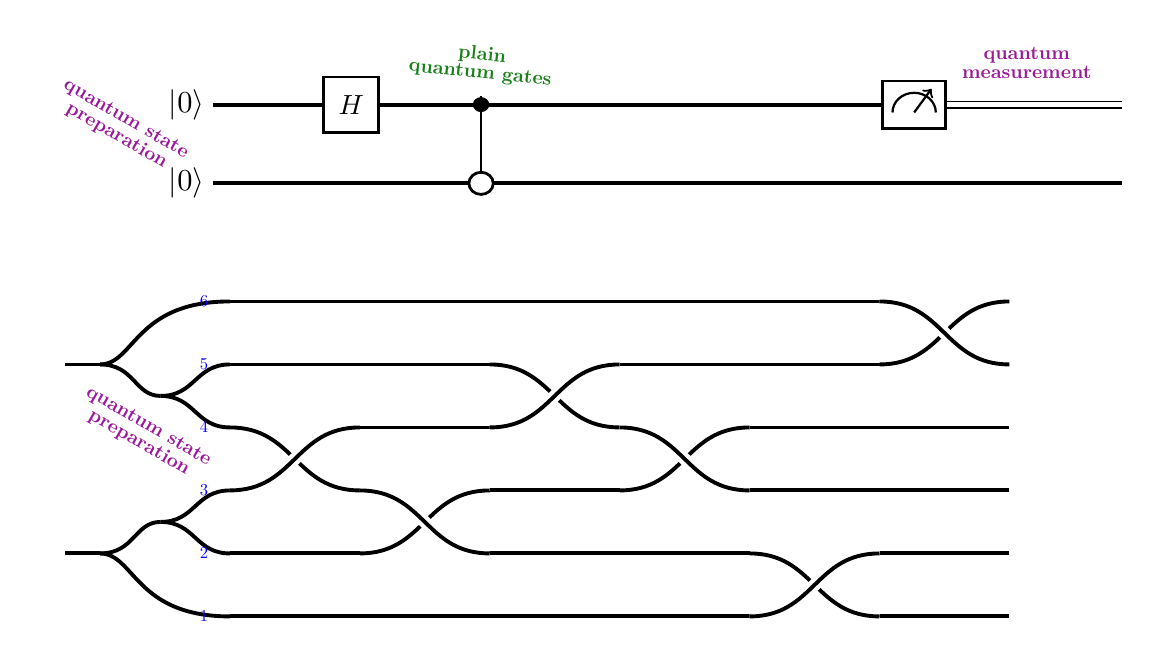
\begin{tikzpicture}[xscale={1.1}]

  \definecolor{purple}{rgb}{0.6, 0.1, 0.6}
  \definecolor{darkgreen}{rgb}{0.1, 0.5, 0.1}
  \definecolor{darkblue}{rgb}{0.1, 0.2, 0.7}

  \draw (-2.8, 0) node { \scalebox{1.1}{$\vert 0 \rangle$} };
  \draw (-2.8, -1) node { \scalebox{1.1}{$\vert 0 \rangle$} };

  \draw[line width=1.5pt] (-2.5,-1) to (+8,-1);
  \draw[line width=1.5pt] (-2.5,0) to (+5.5,0);

  \draw[line width=.6pt] (5.5,+.04) to (8,+.04);
  \draw[line width=.6pt] (5.5,-.04) to (8,-.04);

  \node[draw, fill=white, line width=1pt, minimum width=0.7cm, minimum height=0.7cm] (Hgate) at (-0.9, 0) {$H$};

  \draw[line width=1pt] (0.6, 0) -- (0.6, -1);
  \filldraw[black] (0.6, 0) circle (2.5pt);
  \draw[line width=1pt, fill=white] (0.6, -1) circle (4pt);
  \draw[line width=1pt] (0.6-4pt, -1) -- (0.6+4pt, -1);
  \draw[line width=1pt] (0.6, -1-4pt) -- (0.6, -1+4pt);

  \node[draw, fill=white, line width=1pt, minimum width=0.8cm, minimum height=0.6cm] (MeasBox) at (5.6, 0) {};
  \draw[line width=0.8pt] (5.6-0.25, 0-0.1) arc (180:0:0.25);
  \draw[line width=0.8pt, ->] (5.6, 0-0.1) -- (5.6+0.2, 0+0.2);

  \draw (-3.56, -.3) node[rotate=-30] {
    \scalebox{.7}{\color{purple}\bf\def\arraystretch{.8}\begin{tabular}{c}quantum state\\preparation\end{tabular}}
  };
  \draw (6.9, +.5) node {
    \scalebox{.7}{\color{purple}\bf\def\arraystretch{.8}\begin{tabular}{c}quantum\\measurement\end{tabular}}
  };
  \draw (1-.4, +.5) node[rotate=-6] {
    \scalebox{.7}{\color{darkgreen}\bf\def\arraystretch{.8}\begin{tabular}{c}plain\\quantum gates\end{tabular}}
  };


  \begin{scope}[shift={(-2.3, -4.5)}, rotate=90, yscale=1.0]

    \draw[line width=1.4] (-1.20, 1.90) to (-1.20, 1.50); 
    \draw[line width=1.4] (-1.20, 1.50) .. controls (-1.20, 1.10) and (-2.00, 1.10) .. (-2.00, 0.00); 
    \draw[line width=1.4] (-1.20, 1.50) .. controls (-1.20, 1.10) and (-0.80, 1.10) .. (-0.80, 0.80); 
    \draw[line width=1.4] (-0.80, 0.80) .. controls (-0.80, 0.40) and (-1.20, 0.40) .. (-1.20, 0.00); 
    \draw[line width=1.4] (-0.80, 0.80) .. controls (-0.80, 0.40) and (-0.40, 0.40) .. (-0.40, 0.00); 

    \draw (0.3,1) node[rotate=-30] {
      \scalebox{.7}{\color{purple}\bf\def\arraystretch{.8}\begin{tabular}{c}quantum state\\preparation\end{tabular}}
    };

    \draw[line width=1.4] (1.20, 1.90) to (1.20, 1.50); 
    \draw[line width=1.4] (1.20, 1.50) .. controls (1.20, 1.10) and (0.80, 1.10) .. (0.80, 0.80); 
    \draw[line width=1.4] (1.20, 1.50) .. controls (1.20, 1.10) and (2.00, 1.10) .. (2.00, 0.00); 
    \draw[line width=1.4] (0.80, 0.80) .. controls (0.80, 0.40) and (0.40, 0.40) .. (0.40, 0.00); 
    \draw[line width=1.4] (0.80, 0.80) .. controls (0.80, 0.40) and (1.20, 0.40) .. (1.20, 0.00); 

    \draw (-2.00, 0.3) node {\color{blue}\scalebox{.6}{1}};
    \draw (-1.20, 0.3) node {\color{blue}\scalebox{.6}{2}};
    \draw (-0.40, 0.3) node {\color{blue}\scalebox{.6}{3}};
    \draw (0.40, 0.3) node {\color{blue}\scalebox{.6}{4}};
    \draw (1.20, 0.3) node {\color{blue}\scalebox{.6}{5}};
    \draw (2.00, 0.3) node {\color{blue}\scalebox{.6}{6}};

    \draw[line width=1.4] (-2.00, 0.00) to (-2.00, -1.50);
    \draw[line width=1.4] (-1.20, 0.00) to (-1.20, -1.50);
    \draw[line width=1.4] (1.20, 0.00) to (1.20, -1.50);
    \draw[line width=1.4] (2.00, 0.00) to (2.00, -1.50);
    \draw[line width=1.4] (0.40, 0.00) .. controls (0.40, -0.75) and (-0.40, -0.75) .. (-0.40, -1.50);
    \draw[line width=4.5, white] (-0.40, 0.00) .. controls (-0.40, -0.75) and (0.40, -0.75) .. (0.40, -1.50);
    \draw[line width=1.4] (-0.40, 0.00) .. controls (-0.40, -0.75) and (0.40, -0.75) .. (0.40, -1.50);
    
    \draw[line width=1.4] (-2.00, -1.50) to (-2.00, -3.00);
    \draw[line width=1.4] (0.40, -1.50) to (0.40, -3.00);
    \draw[line width=1.4] (1.20, -1.50) to (1.20, -3.00);
    \draw[line width=1.4] (2.00, -1.50) to (2.00, -3.00);
    \draw[line width=1.4] (-1.20, -1.50) .. controls (-1.20, -2.25) and (-0.40, -2.25) .. (-0.40, -3.00);
    \draw[line width=4.5, white] (-0.40, -1.50) .. controls (-0.40, -2.25) and (-1.20, -2.25) .. (-1.20, -3.00);
    \draw[line width=1.4] (-0.40, -1.50) .. controls (-0.40, -2.25) and (-1.20, -2.25) .. (-1.20, -3.00);
    
    \draw[line width=1.4] (-2.00, -3.00) to (-2.00, -4.50);
    \draw[line width=1.4] (-1.20, -3.00) to (-1.20, -4.50);
    \draw[line width=1.4] (-0.40, -3.00) to (-0.40, -4.50);
    \draw[line width=1.4] (2.00, -3.00) to (2.00, -4.50);
    \draw[line width=1.4] (1.20, -3.00) .. controls (1.20, -3.75) and (0.40, -3.75) .. (0.40, -4.50);
    \draw[line width=4.5, white] (0.40, -3.00) .. controls (0.40, -3.75) and (1.20, -3.75) .. (1.20, -4.50);
    \draw[line width=1.4] (0.40, -3.00) .. controls (0.40, -3.75) and (1.20, -3.75) .. (1.20, -4.50);
    
    \draw[line width=1.4] (-2.00, -4.50) to (-2.00, -6.00);
    \draw[line width=1.4] (-1.20, -4.50) to (-1.20, -6.00);
    \draw[line width=1.4] (1.20, -4.50) to (1.20, -6.00);
    \draw[line width=1.4] (2.00, -4.50) to (2.00, -6.00);
    \draw[line width=1.4] (-0.40, -4.50) .. controls (-0.40, -5.25) and (0.40, -5.25) .. (0.40, -6.00);
    \draw[line width=4.5, white] (0.40, -4.50) .. controls (0.40, -5.25) and (-0.40, -5.25) .. (-0.40, -6.00);
    \draw[line width=1.4] (0.40, -4.50) .. controls (0.40, -5.25) and (-0.40, -5.25) .. (-0.40, -6.00);
    
    \draw[line width=1.4] (-0.40, -6.00) to (-0.40, -7.50);
    \draw[line width=1.4] (0.40, -6.00) to (0.40, -7.50);
    \draw[line width=1.4] (1.20, -6.00) to (1.20, -7.50);
    \draw[line width=1.4] (2.00, -6.00) to (2.00, -7.50);
    \draw[line width=1.4] (-1.20, -6.00) .. controls (-1.20, -6.75) and (-2.00, -6.75) .. (-2.00, -7.50);
    \draw[line width=4.5, white] (-2.00, -6.00) .. controls (-2.00, -6.75) and (-1.20, -6.75) .. (-1.20, -7.50);
    \draw[line width=1.4] (-2.00, -6.00) .. controls (-2.00, -6.75) and (-1.20, -6.75) .. (-1.20, -7.50);
    
    \draw[line width=1.4] (-2.00, -7.50) to (-2.00, -9.00);
    \draw[line width=1.4] (-1.20, -7.50) to (-1.20, -9.00);
    \draw[line width=1.4] (-0.40, -7.50) to (-0.40, -9.00);
    \draw[line width=1.4] (0.40, -7.50) to (0.40, -9.00);
    \draw[line width=1.4] (1.20, -7.50) .. controls (1.20, -8.25) and (2.00, -8.25) .. (2.00, -9.00);
    \draw[line width=4.5, white] (2.00, -7.50) .. controls (2.00, -8.25) and (1.20, -8.25) .. (1.20, -9.00);
    \draw[line width=1.4] (2.00, -7.50) .. controls (2.00, -8.25) and (1.20, -8.25) .. (1.20, -9.00);

  \end{scope}

\end{tikzpicture}
\caption{ A standard $2$-qubit quantum circuit and its lowering to a braid-circuit with
  inection weaves (missing yet).}
\end{figure}

\subsection{Application: Evaluating the Jones Polynomial}